%%==========================
%% chapter01.tex for TJU Master Thesis
%% based on CASthesis
%% modified by charlie.yaha@gmail.com
%% version: 0.1alpha
%% Encoding: UTF-8
%% last update: Dec 5th, 2010
%%==================================================

%\bibliographystyle{TJU} %[此处用于每章都生产参考文献]


\chapter{绪~论}
\label{chap:introduintroduction}
\section{研究背景}



液压系统是航空航天等产品的重要系统之一。
现代飞机航面操纵系统与动力收放系统几乎都是液压驱动的。液压系统作为飞机飞行控制系统和起落架等负载的动力源,对飞机的安全飞行起着关键的作用。
大型客机的液压系统,是一个多余度、大功率的复杂综合系统,控制着飞机起落架、襟翼、减速板的收放,平尾、副翼、方向舵的操纵,进气锥、辅助进气门的调节等\cite{dingfei2010}。空客的A320,波音的B737都配备了至少3套相互独立的液压\cite{dingfei2010},多套液压系统相互独立、相互备份,管线密布机身,如图\ref{fig:plane-hose}所示,管线长度一般在机身长度的数倍以上。液压系统的各类管线,是现代航空航天工业中即为重要的部件之一。

\begin{figure}[!htbp]
	\centering
	%	\subfigure[起落架]{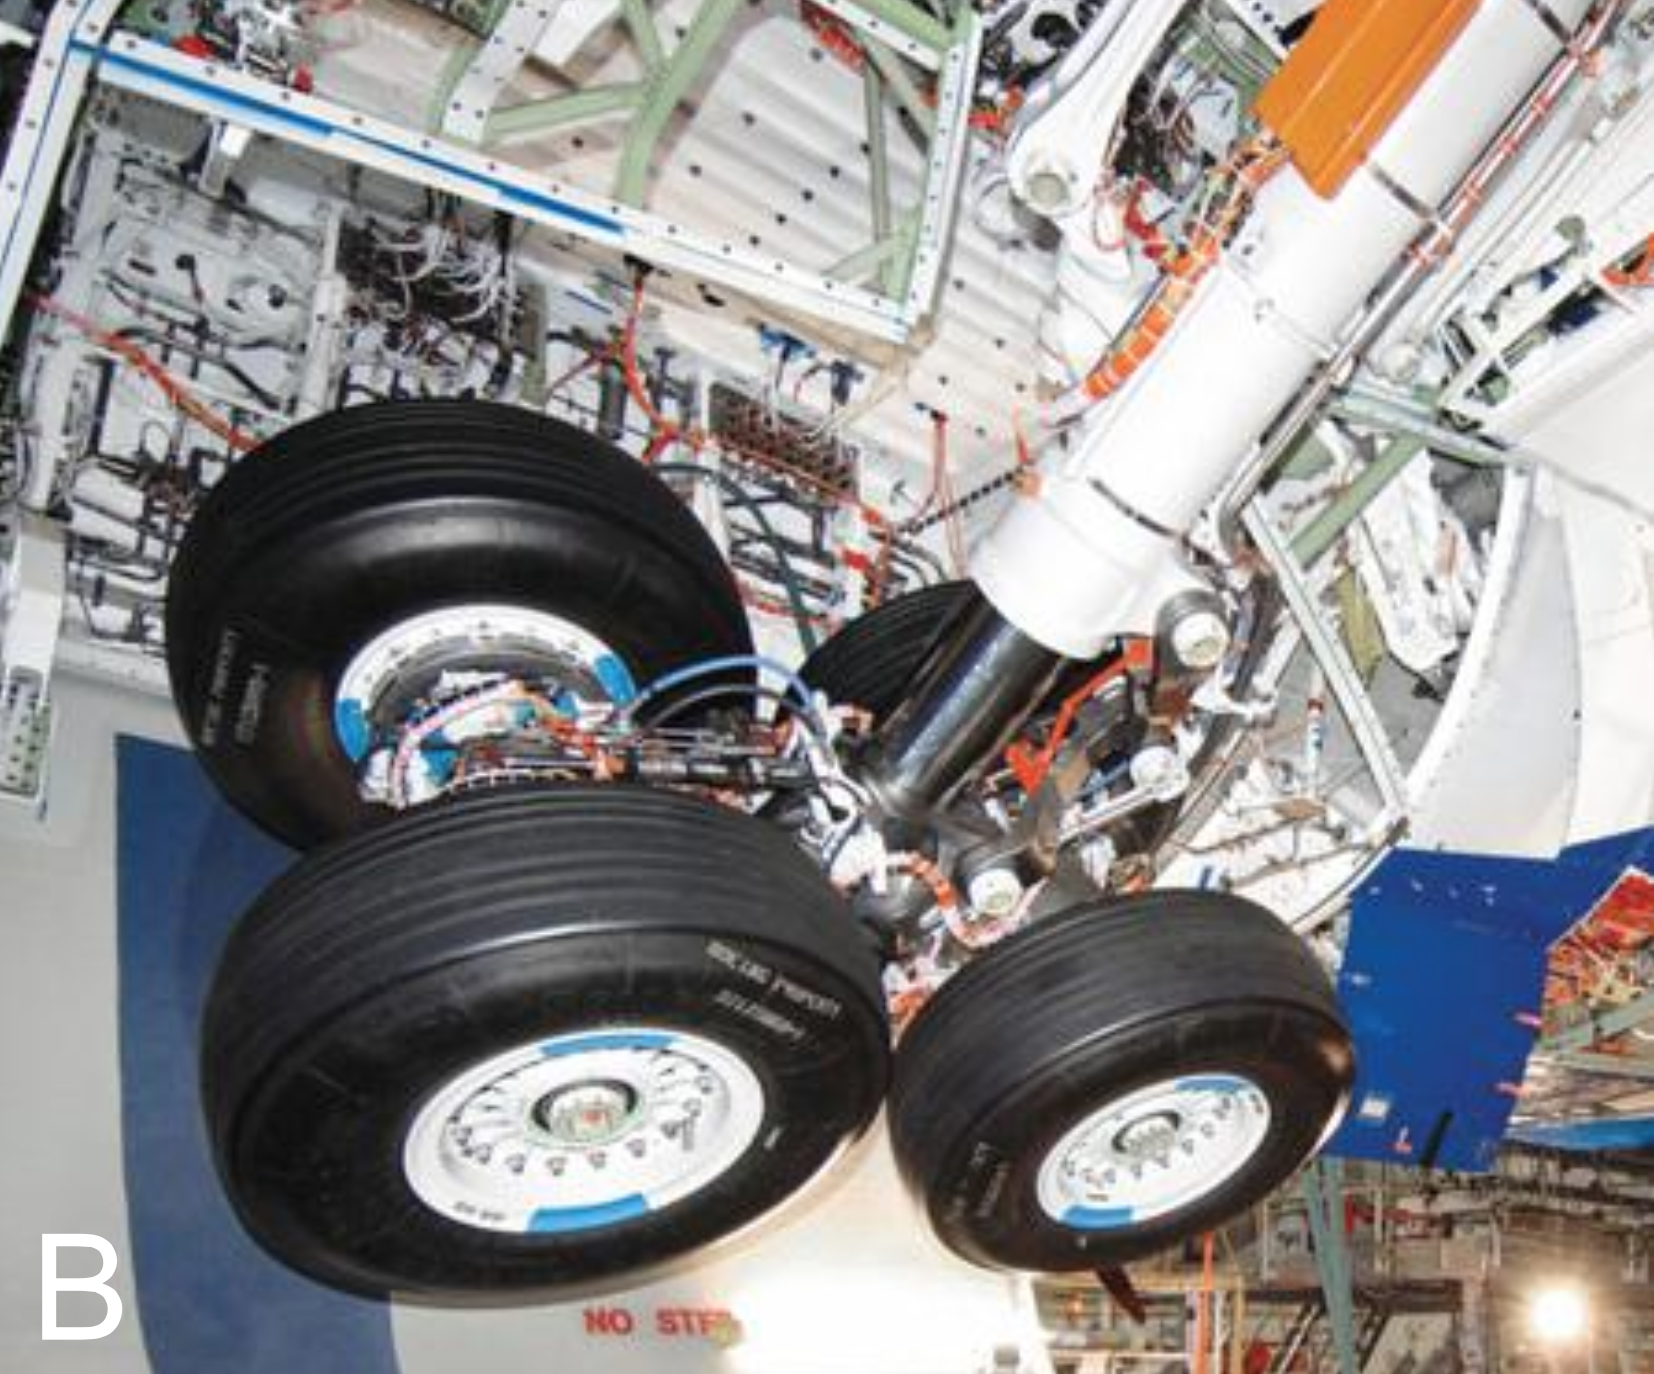
\includegraphics[width=0.4\textwidth]{figure/chap1/gear}}		\label{fig:plane gear}
	%	\hspace{1cm}
	%	\subfigure[飞机管路]{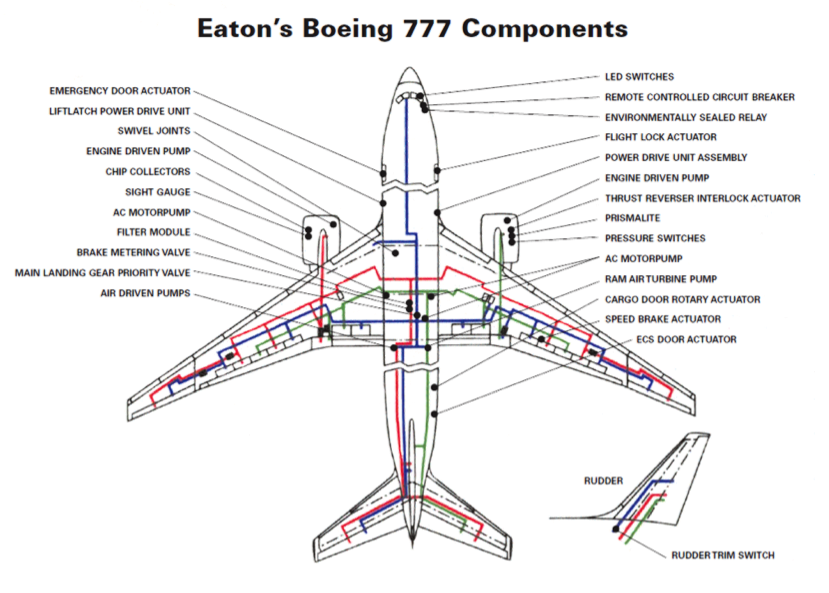
\includegraphics[width=0.5\textwidth]{figure/chap1/Plane}}    \label{fig:plane}
	\subfigure[机身软管管路(a.软管,b.液压源)]{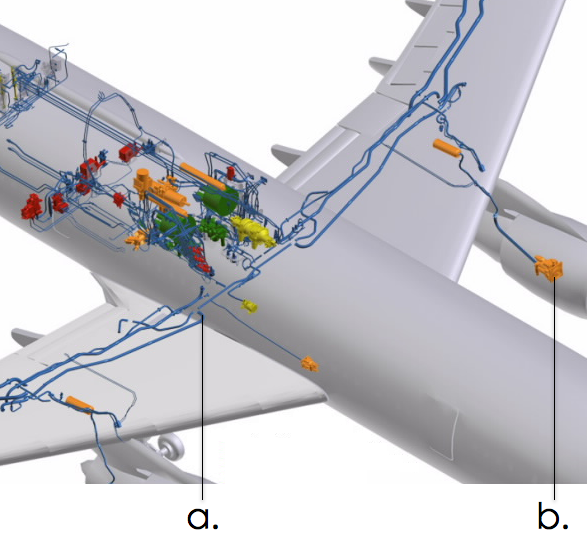
\includegraphics[width=0.4\textwidth]{figure/chap1/plane-cruit}\label{fig:plane-cruit}}    
	\hspace{1cm}
	\subfigure[发动机软管管路(a.软管,b.液压源)]{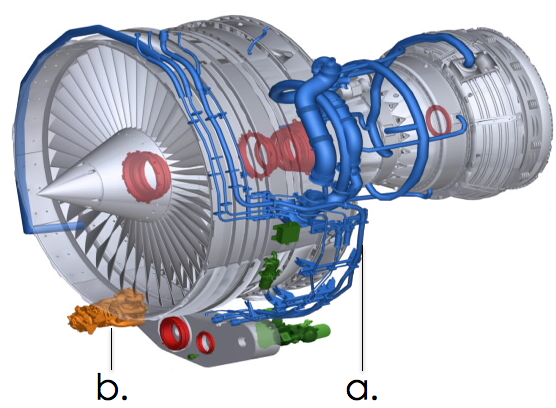
\includegraphics[width=0.4\textwidth]{figure/chap1/engine-cruit}\label{fig:engine-cruit}}    
	\bicaption[fig:Distribution of hose assembly]{飞行器液压系统管线分布}{飞行器液压系统管线分布}{Fig}{Distribution of hose assembly in a plane}  
	\label{fig:plane-hose}
\end{figure}




现代飞机液压系统大多采用变量柱塞泵,脉动式的流量输出是其固有特性;同时液压系统工作时,在阀门打开或关闭的瞬间,供压管路和回油管路会出现强烈的压力撞击,即压力脉冲。变量柱塞泵产生的压力脉动,在高速、高压、高温、大流量条件下,若与系统匹配不当,油泵出口压力会产生高频等幅振荡,从而很容易导致两种耦合振动:一种是脉动频率与流体谐振频率接近时的耦合振动;另一种是脉动频率与管路系统结构的固有频率接近时,发生的耦合振动。
在高压管路上,压力脉冲峰值有可能达到系统额定压力的1.5倍以上,而在回油管路上则可能达到正常回油压力值的10倍以上\cite{lijun2007}。
这种脉冲峰值很容易导致管壁破裂、管路支撑结构破坏,引起支撑刚度下降、管路系统失效、液压油液泄露,从而导致严重的灾难性事故\cite{gaofeng2013}。


据统计,当前我国飞机液压系统的故障约占飞机机械系统总故障的$ 30\%$左右,飞机液压系统的维修工作量占机械维修工作量的$1/3 $\cite{lijun2007},而液压系统的故障几乎都发生在管路部分。
例如,我国七十年代研制的某机型,从油泵出口至蓄压器之间的软管管路不断发生断裂,影响到设计定型;
八十年代初,我国研制的某型号机地面试车时,由于液压软管爆裂引发大火,致使整架飞机毁于一旦,不仅造成巨大的经济损失,而且使型号研制进度推迟了两年;某型机的泵出口软管出现多次爆裂事故,由于管路断裂,液压系统失效,发生了飞机启用应急系统、强迫着陆及驾驶员应急跳伞等严重问题\cite{lijun2007,guoqing2010,gaofeng2013}。

\begin{figure}
	\centering
	\subfigure[波音b777起落架液压软管]{
		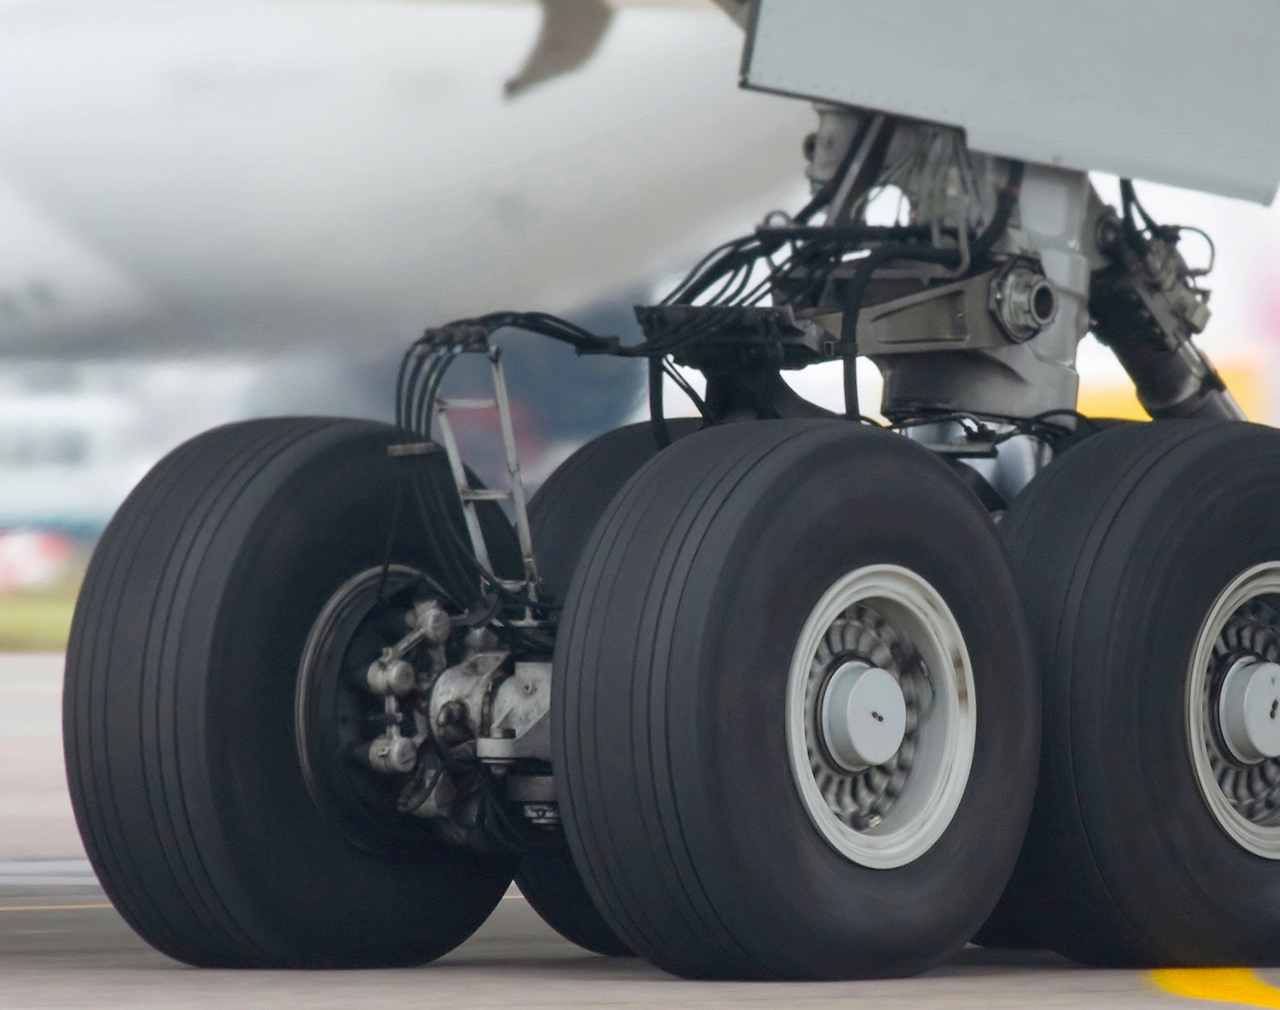
\includegraphics[width=0.4\textwidth]{figure/chap1/777-gear}\label{fig:777-gear}}
	\hspace{1cm}
	\subfigure[a380起落架液压软管]{
		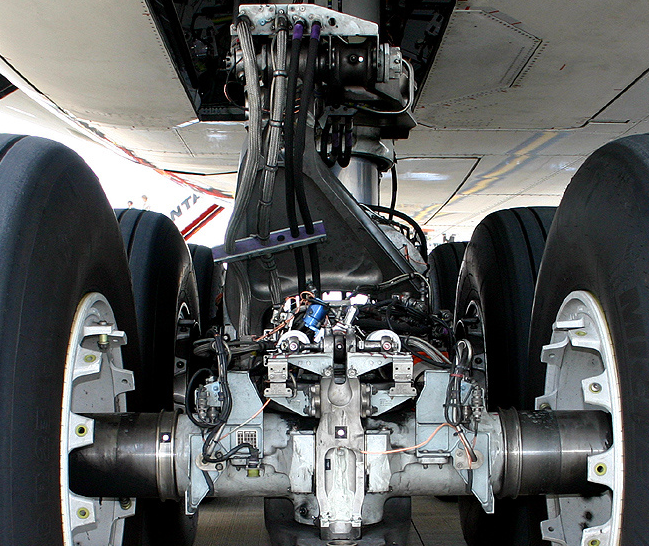
\includegraphics[width=0.4\textwidth]{figure/chap1/a380-gear}\label{fig:a380-gear}}
	\bicaption[fig:gear hose cruit]{起落架软管管路}{起落架软管管路}{Fig}{Hydraulic hose cruit of gear}  
	\label{fig:plane-hose}
\end{figure}



因为液压泵出口处的高频振动,刚性管受激共振而破坏失效,必须要低刚度的柔性管来吸收振动的能量,
同时因为飞机液压能源系统由于飞机对空间和质量的限制,常常具有一般管路设计中需要避免的长跨度、低刚度管段出现\cite{gaofeng2013}。
因此,飞机动作控制液压系统(\ref{fig:plane-cruit})以及飞机引擎液压、燃油系统(\ref{fig:engine-cruit})中,大量的管道并非刚性管,而是由大量柔性软管组成的。


随着航空技术的不断发展,飞机液压系统也在向高压化、大功率的方向发展。
因为提高飞机的液压系统工作压力是减小系统自身重量和体积的重要手段。
空客A320液压系统额定工作压力为3000psi(21MPa)
最新的客机型号波音的B787和空客A380的的液压系统压力等级都达到 5000psi(35MPa)\cite{lavooij1991},
国外领先企业Eaton Aerospace、Parker Hannfin公司也已经为军用飞机开发出来8000psi(55MPa)的液压泵,空客公司也已经提出了将起落架刹车制动液压管路工作压力提高到8000psi(55MPa)的目标,而国内的液压系统一般只能做到3000psi(21MPa)。


\begin{figure}
	\centering
	\subfigure[软管失效]{
		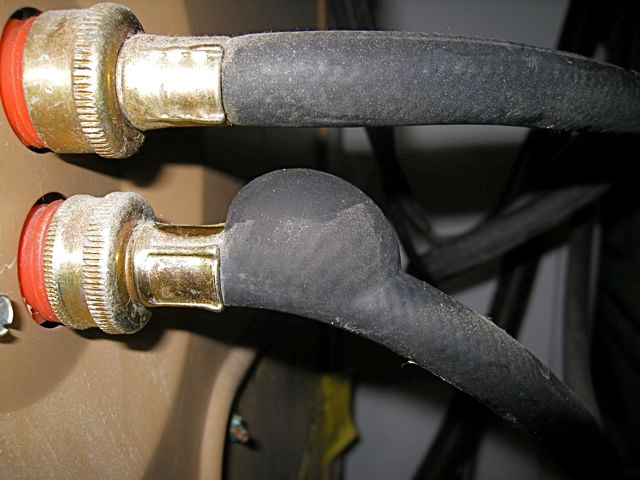
\includegraphics[width=0.4\textwidth]{figure/chap1/burst-hose-1}}
	\hspace{1cm}
	\subfigure[软管失效]{
		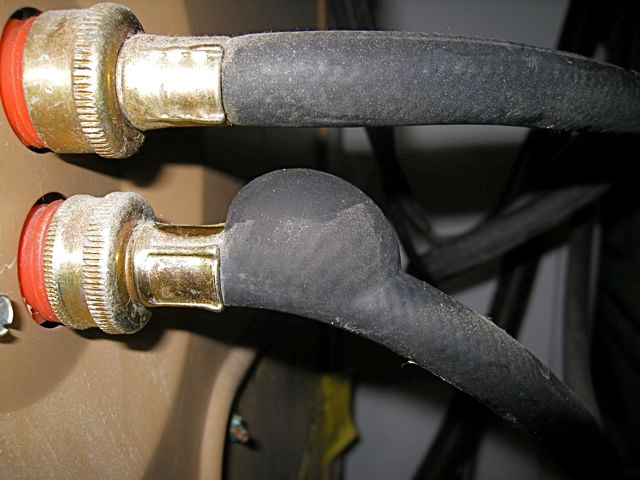
\includegraphics[width=0.4\textwidth]{figure/chap1/burst-hose-1}}
	\bicaption[fig:hose burst]{软管失效}{软管失效}{Fig}{hose fail}  
	\label{fig:plane-hose}
\end{figure}





液压泵脉动控制方面,国内液压泵一般流量脉动为$\pm10\%$,国外一般在$ \pm5\% $左右\cite{lijun2007}。Eaton公司为空客A380最新研制出一种内置衰减器的柱塞泵,压力脉动变化为$ \pm 1\%$。可见国内液压泵脉动控制的水平距国际先进水平尚有一定距离。而飞机液压系统的压力脉冲是造成液压元件提前损坏,导致液压系统故障的主要原因之一。考虑到新型柱塞泵的研发周期,目前能够有效提高液压系统可靠性的办法,就是提升液压软管的设计、生产水平。

目前国内液压软管的设计水平尚处于仿造阶段,参考的是美国SAE-J517液压软管标准。国内产品试制基本依靠经验结合实验,以美国制定的一系列MIL-H-25579E、SAE AS604、SAE AS614等软管脉冲试验标准,作为为检验标准。
国外美国、俄罗斯、日本和国际标准化组织,都在液压软管脉冲试验方面起步较早,已经有成熟的规范、标准试验设施和完整的试验方法。
而我国对于液压软管脉冲试验研究起步较晚,这方面仍然是一个空白。













%了解什么事软管
\section{软管组件简介}
%软管定义,软管组件结构
编织加强软管由内管、纤维增强层及金属连接件组成,是一种复合结构的管路连接件,一般将整个系统结构称为软管组件(Flexible Hose Assembly),或软管总成(本文统一称为软管组件)。
其结构如图\ref{fig:hose structure}所示:柔性内管,例如橡胶管,氟塑料管,热塑料管,金属波纹管,其外外包覆若干层柔性加强结构(编织、缠绕),主要承受内管的内压荷载,加强层数一般视内压荷载大小而定。软管组件工作时,绝大部分内压荷载由编织层承担,内管主要起通道的作用。


\begin{figure}[!htbp]
\centering
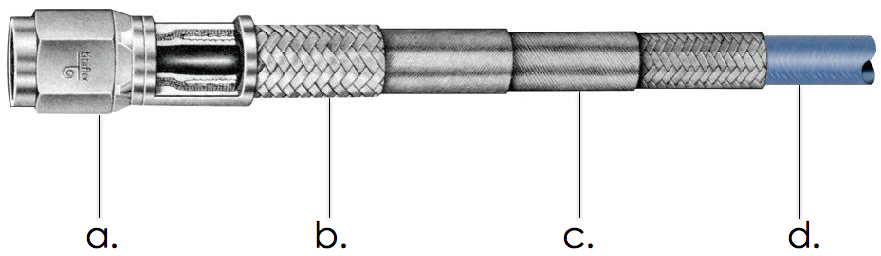
\includegraphics[width=0.6\linewidth]{figure/chap1/Hose-Structure}
\bicaption[fig:hose structure]{软管组件结构}{软管组件结构(a.接头,b.金属纤维编织层,c.金属纤维缠绕层,d.内管)}{Fig}{Hose Structure(a.Coupling,b.Braid Layer,c.Helix-wound Layer,d.Inner Tube)}
\label{fig:hose structure}
\end{figure}


软管组件主要应用于液压、气动、燃油、滑油等系统的介质传输,起到了“血管”作用,航空航天飞行器、汽车、船舶,以及各种工业设备、机床等,都大量使用了软管组件。如图\ref{fig:plane-hose}所示,飞机液压系统(\ref{fig:plane-cruit})



%在刚性管无法使用的情况下使用:
%\begin{itemize}
%	\item 持续的运动
%	\item 振动
%	\item 冲击
%	\item 任意排列
%	\item 高压和压力的释放
%\end{itemize}

软管组件是液压传动系统中非常重要的组成部分。相比普通硬质管,软管组件可以承受相对较大的内压、轴向荷载,同时保持较小的质量、弯曲刚度,带来以下优势:可以减小系统的刚度,吸收液压源产生的振动;安装方式灵活,节约了系统内部的空间。




%软管优势



%不同软管型号
软管组件根据不同的口径、编织加强层的层数、重量等参数有以下分类方法:重型、中型、轻型;低压、中压、高压。
重型管管径一般达到20mm,轻型管管径一般在10mm以下;
高压管一般爆破压力要求达到\SI{80}{\mega\pascal},低压管爆破压力一般在40MPa以下。
不同型号的软管对于着不同的工作环境,如以下表\ref{tab:hosefixposition}所示,




\begin{table}[!htbp]
	\centering
	\bicaption[tab:hosefixposition]{不同型号软管组件安装位置}{不同型号软管组件安装位置}{Fig}{Position}
		
	\begin{tabular}{ccc}
		\toprule
		&    轻型     &     重型     \\ \hline
		低压 & 汽车刹车、转向传动 &  输运水、气  \\
		高压 & 飞机起落架、襟翼  & 飞机、船舶液压泵出口 \\ 
		\bottomrule
	\end{tabular} 
\end{table}

%解释表格
飞机、船舶液压泵出口处压强高,流量大,震动强,工作环境极为恶劣,因此国内外一般都采用重型高压软管组件,技术也都已经较为成熟。
飞机起落架、襟翼等部位处于机身液压系统的末端,但压强仍然很高,而且软管的安装空间很小,要求软管组件具有较小的弯曲半径。保持较高的爆破压力的同时,使得软管组件小型化、轻型化,这就对软管组件的设计水平提出了很高的要求。国外企业在轻型高压软管组件领域技术优势明显,基本垄断了该市场。

汽车领域也大量使用了软管组件,例如刹车制动管,转向传动管,空调管等。相比飞行器的液压系统,汽车的液压系统压强较低,如刹车制动管的爆破压力一般为35MPa至40MPa\footnote{GB 16897-2010}。但汽车行业对成本较为敏感,要求在保证设计指标的同时,使软管的结构达到最优化。这对软管的设计、制造也提出了很高的要求。

%软管材质
根据软管寿命、工作环境温度

 	 	 
					
\section{软管组件研究现状}

软管组件的加工生产技术经过几次重大变革,至今为止,已经发展出了3代产品。
金属增强软管组件是由美国发明并于上世纪60年代开始用于飞机的液压系统,
%第一代
在此之前为第一代软管组件,以橡胶软管为主;

从上世纪60年代到上世纪90年代中期,
第二代金属加强软管已经广泛应用于航空、航天领域。同时也根据不同的压力等级需求和工作环境发展出不同的加强形式,如编织加强、缠绕加强;也发展出了不同的内管材料,如PTFE氟塑料、热塑料、尼龙等;还出现了防火、防磨损、防腐蚀、防紫外线等各式附件,品种繁多。
为此,美国建立了一系列的军用、宇航产品技术标准或规范,例如:MIL-H-25579E、SAE AS604、SAE AS614等。
第二代软管组件的最高使用温度已达232\textcelsius,最高工作压力已经达55MPa。
已经广泛应用于各种类型的飞机和导弹、运载火箭等,例如:F-16、F-22、波音客机等。


%第三代
近年来,航空航天事业飞速发展,对软管组件也提出轻量化的要求,传统钢丝增强软管组件已不能满足航空航天的设计要求。
为了解决这个问题,美国Titeflex、Eaton及Parker等国际知名公司,已在20世纪80年代,开始了第三代软管组件——非金属增强软管组件的研究。他们纷纷研制推出了各自的非金属增强软管组件产品。目前波音B787就大量使用了Eaton公司的AS1975以及AS4623 Kevlar加强软管组件,满足5080psi(35MPa)工作压力要求。


目前对金属编织加强软管的研究,多见于汽车工业中的中刹车管[2]、转向传动管[3]、空调管[4]等。对软管加强层理论的研究,基本使用通过加强层的总体的要是通过软管理论主要有两个分支[5]:一种是加强层含量较低,橡胶管起主要作用的软管,由Kuipers等人[6,7]提出并完善,适用于帘线加强的软管;另一种是编织加强层主要承力的软管,主要研究的是钢丝螺旋缠绕加强层。软管轴向受拉时,缠绕的金属丝会沿缠绕方向“流动”。编织加强层仅作为螺旋缠绕的一种特例:两层缠绕方向相反,且不允许“流动”的缠绕层[5]。
近20年对编织加强结构的研究主要集中在复合材料编织。复合材料纤维编织的与金属纤维编织的传力机制差别非常明[8]:复合材料纤维只承受单向应力;而金属编织层中的金属丝间的接触关系会直接影响编织层整体的传力,不能忽视。因此,并没有至今尚没有成熟、独立,考虑金属丝间接触关系的编织加强层理论。
有学者尝试用连续介质力学的基本理论推导编织层的本构,如Evans[5]编织层金属纤维侧向传力机制,Horgan等人[9]提出了纤维加强材料的应变能密度函数,国内学者计算了编织结构强度与突加荷载的情况[10,11]。但主流的研究办法还是结合实验,提出能够反映加强层力学行为的有限元模型。Wijaya[4]对包含软管各层材料及编织层的试件进行了压缩实验,认为金属编织层的应力应变关系是线性的,在软管整体动态特性的研究中取得了较好的效果。Cho[3]研究了编织层在扣压安装接头中的力学行为,结合压缩实验提出了弹塑性的本构模型,Rattensperger[8]同样针对压缩的过程,编织层厚度方向引入一组等效非线性弹簧,表征金属纤维间相互作用。
Hachemi[12]对编织层进行了拉伸试验,将复合材料编织中考虑材料非线性行为的特征单元法(首先由Reese[13]提出)引入金属编织层的研究,提出了能够反映编织结构编织角变化的本构模型。该模型将编织层简化两层Rebar单元,只在编织方向上有刚度。但该模型仍然没有考虑两层Rebar单元之间相互接触的关系。

\section{研究内容}
本研究实验表明,Hachemi[12]本构模型的非线性行为并不足够强,不能与本研究中的高压金属编织加强软管的拉伸实验结果相吻合。我们试图通过引入金属纤维间的接触关系来修正该理论与实验的差距。使得包括非线性段的实验结果都能够与修正后的理论值相吻合。
 
